
C++20是继C++11之后的一个重要的标准。像C++11一样,C++20也会改变了我们使用现代C++编程的方式。这种变化主要在于在中添加了概念、模块、范围和协程等特性。为了了解C++发展的下一步,先在这里简单介绍一下有C++20的历史背景。

\begin{center}
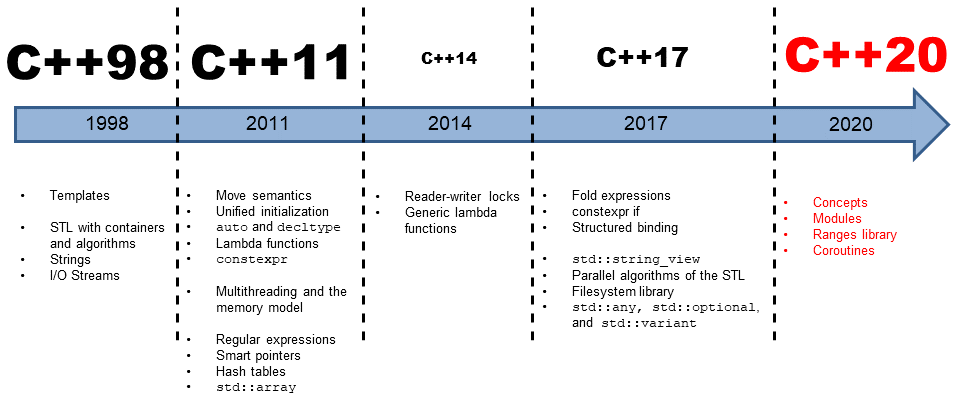
\includegraphics[width=1.0\textwidth]{content/1/chapter1/images/1.png}\\
C++的历史
\end{center}

C++出现已经有40年了,以下是对过去几年变化的简要概述。





























